\begin{figure}[h] 
\centering
\begin{subfigure}[b]{0.225\textwidth}
	\centering
	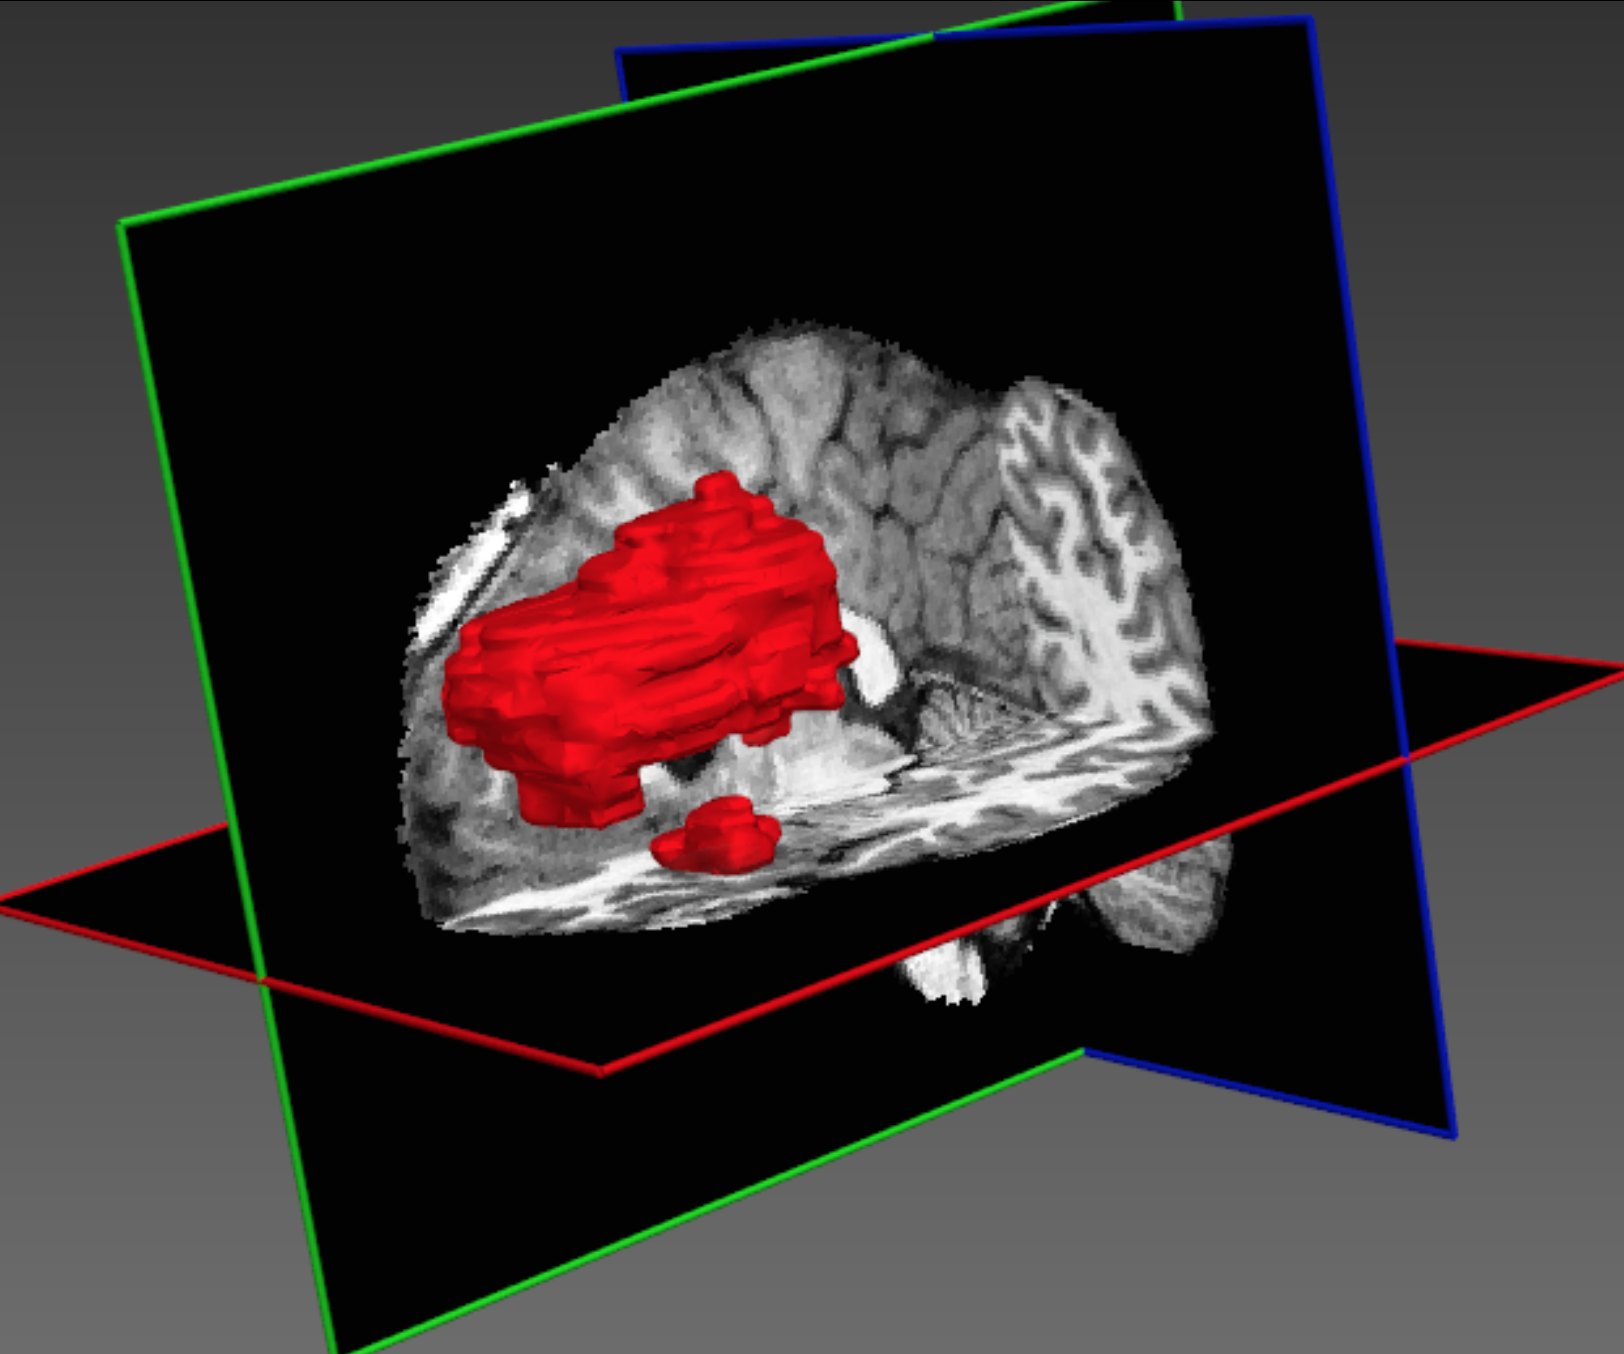
\includegraphics[clip=true, trim=10pt 0pt 10pt 0pt, width=1.\textwidth]{figures/introduction/3dLesionBig.png}
	\caption{}
	\label{fig:3dLesionBig}
\end{subfigure}
\begin{subfigure}[b]{0.225\textwidth}
	\centering
	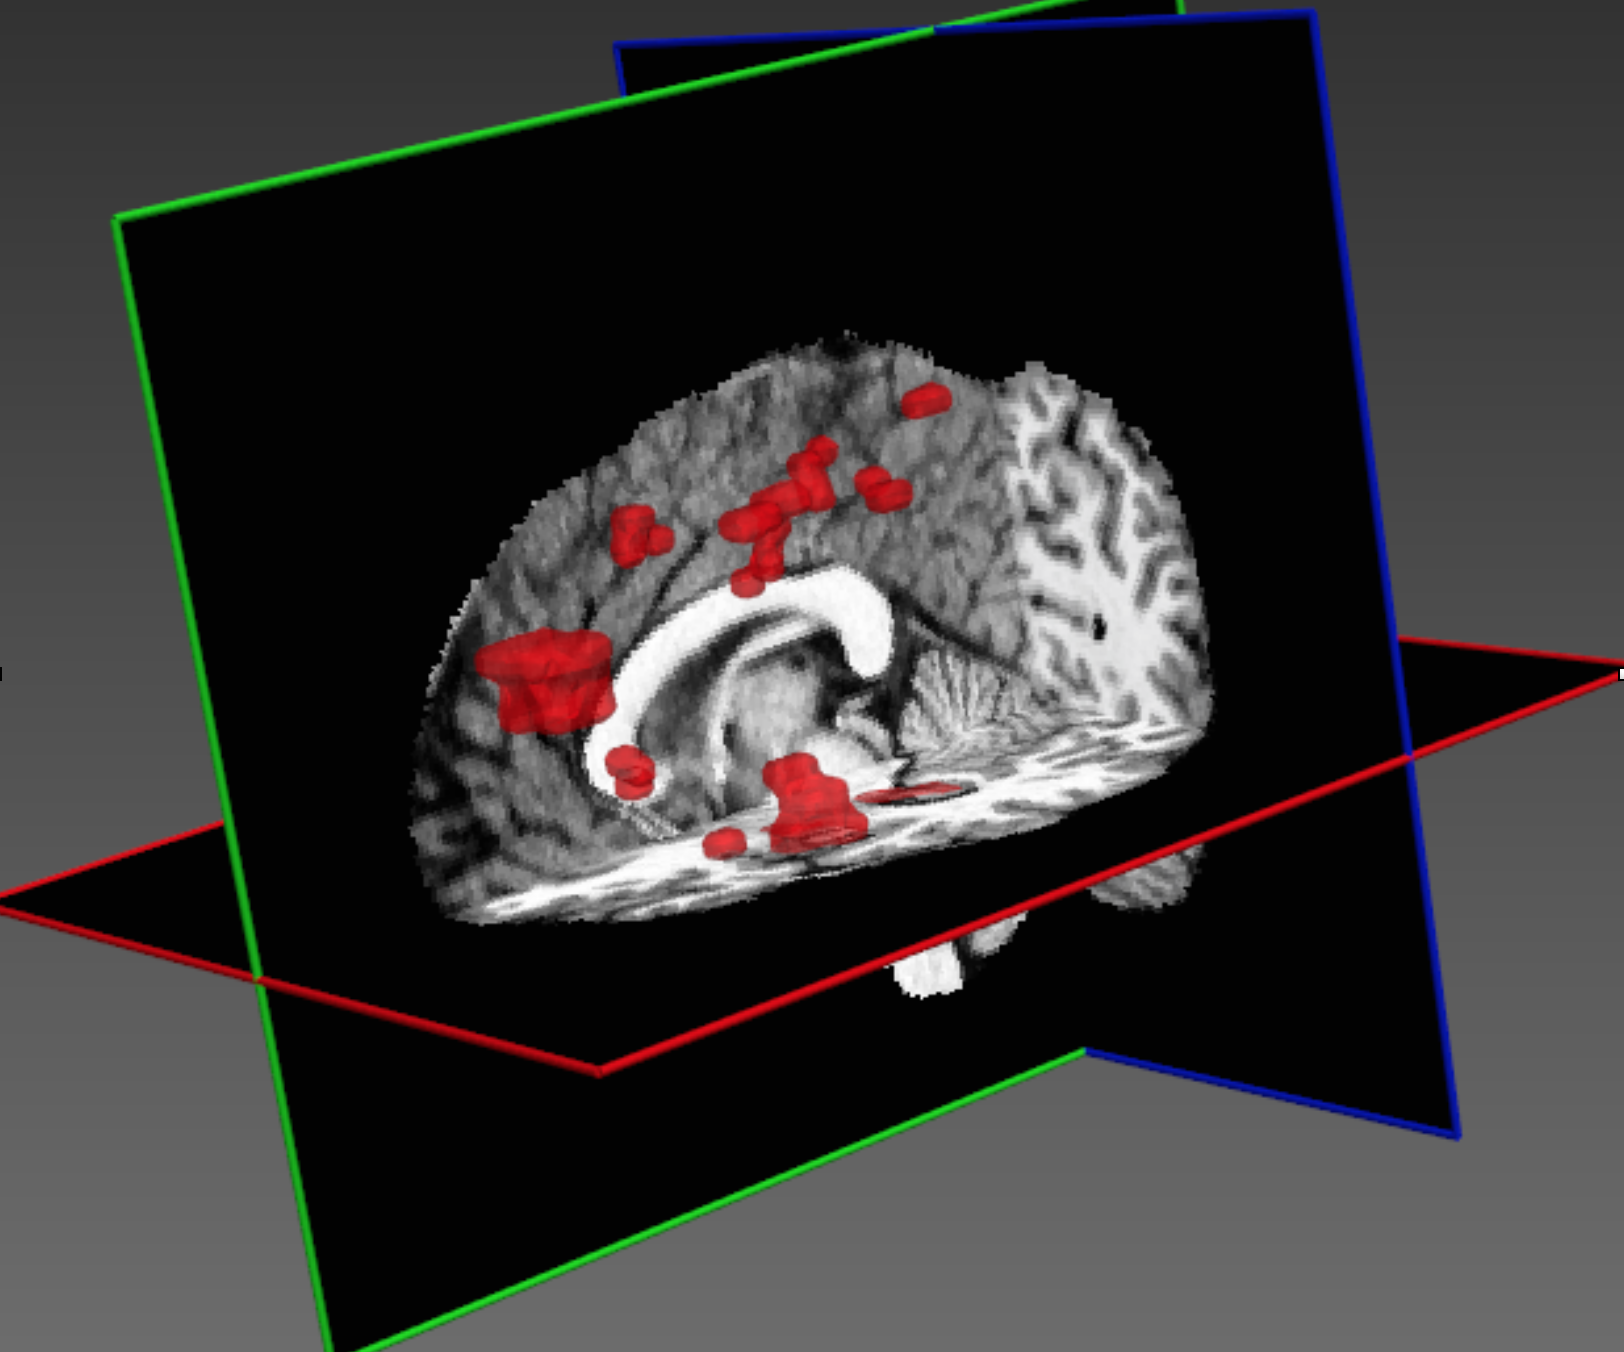
\includegraphics[clip=true, trim=10pt 0pt 10pt 0pt, width=1.\textwidth]{figures/introduction/3dLesionsSmalls.png}
	\caption{}
	\label{fig:3dLesionSmalls}
\end{subfigure}
\begin{subfigure}[b]{0.225\textwidth}
	\centering
	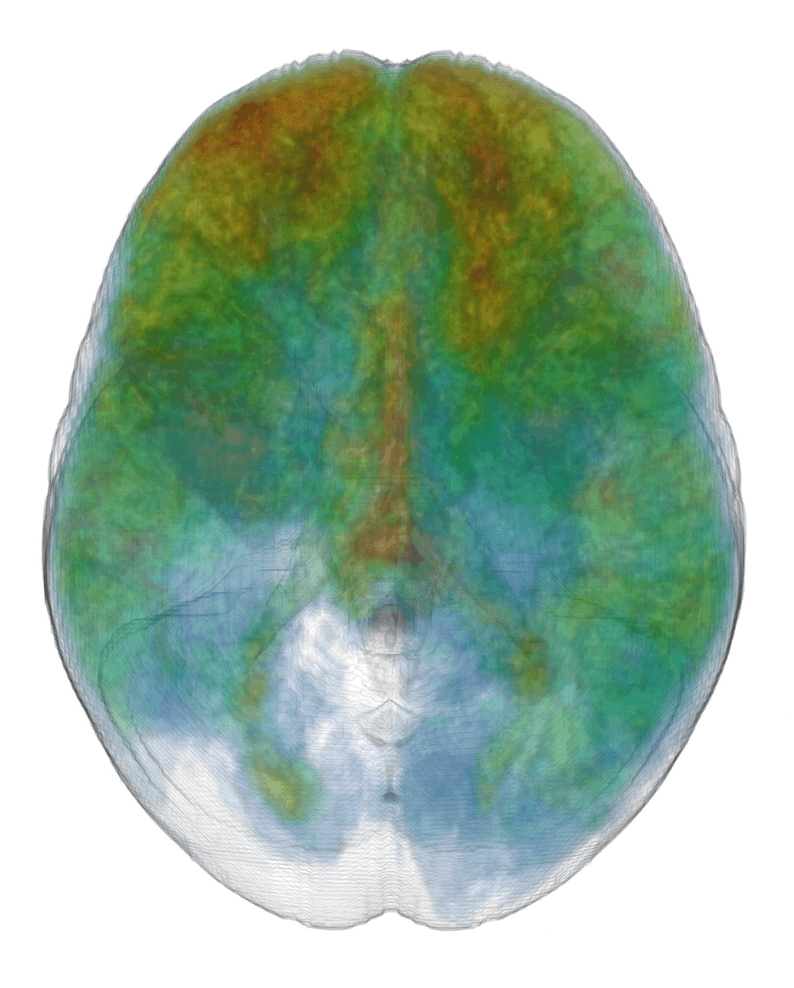
\includegraphics[clip=true, trim=10pt 20pt 10pt 20pt, width=0.7\textwidth]{figures/introduction/trio/top1Small.png}
	\caption{}
	\label{fig:spatialMap}
\end{subfigure}
\begin{subfigure}[b]{0.22\textwidth}
	\centering
	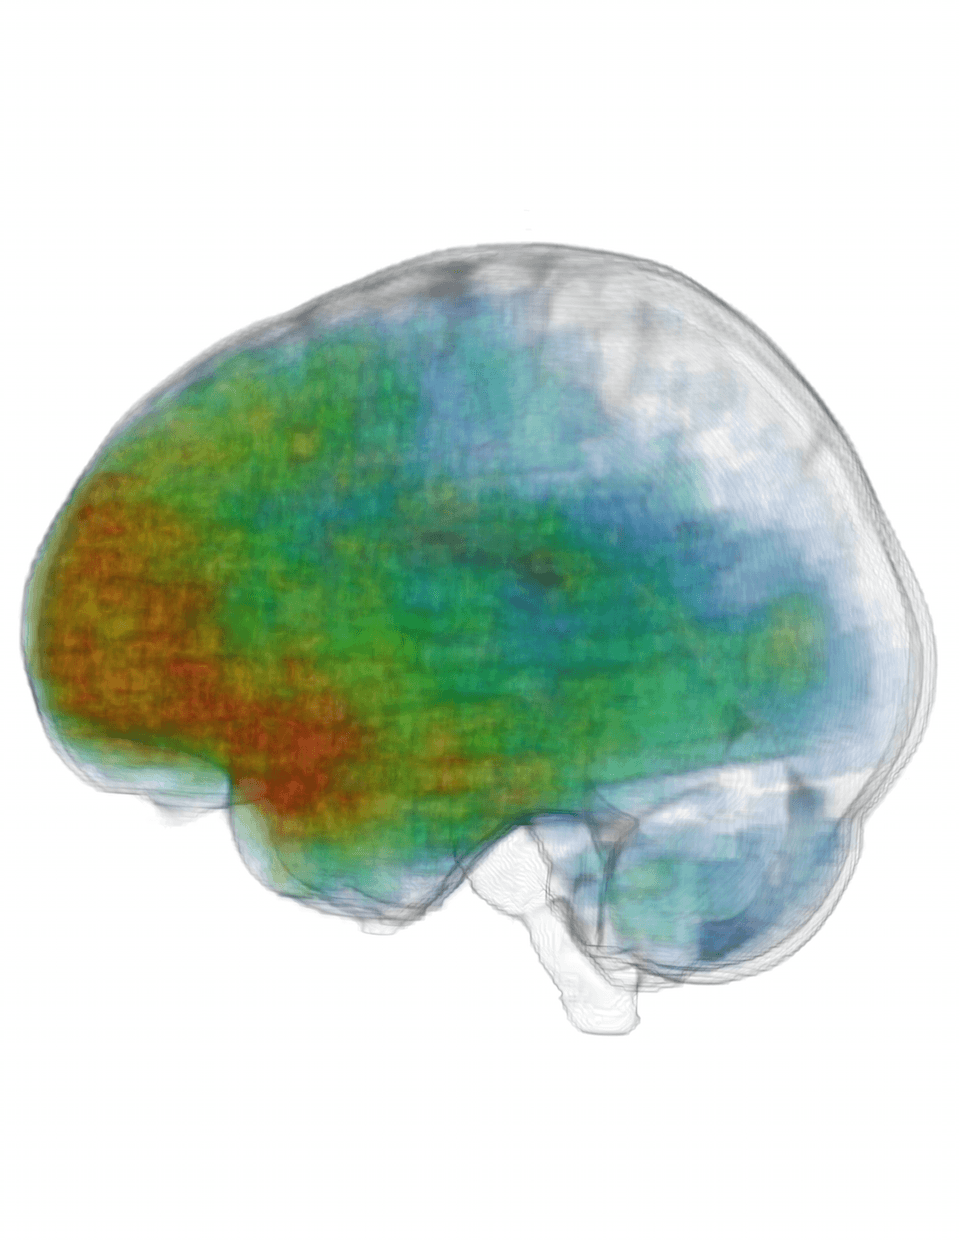
\includegraphics[clip=true, trim=0pt 190pt 0pt 0pt, width=1.0\textwidth]{figures/introduction/trio/side1Small.png}
	\caption{}
	\label{fig:spatialMapSide}
\end{subfigure}
%add desired spacing between images, e. g. ~, \quad, \qquad, \hfill etc.
%(or a blank line to force the subfigure onto a new line)
\\[1ex] %Break line. So that next figures go in their own line.
\centering
\begin{subfigure}[b]{1.0\textwidth}
\centering
	%\includegraphics[width=1.0\textwidth]{figures/figIntHistoWholeDataset/new13Mar/histoIntensGreenRedNoSupt.png}
	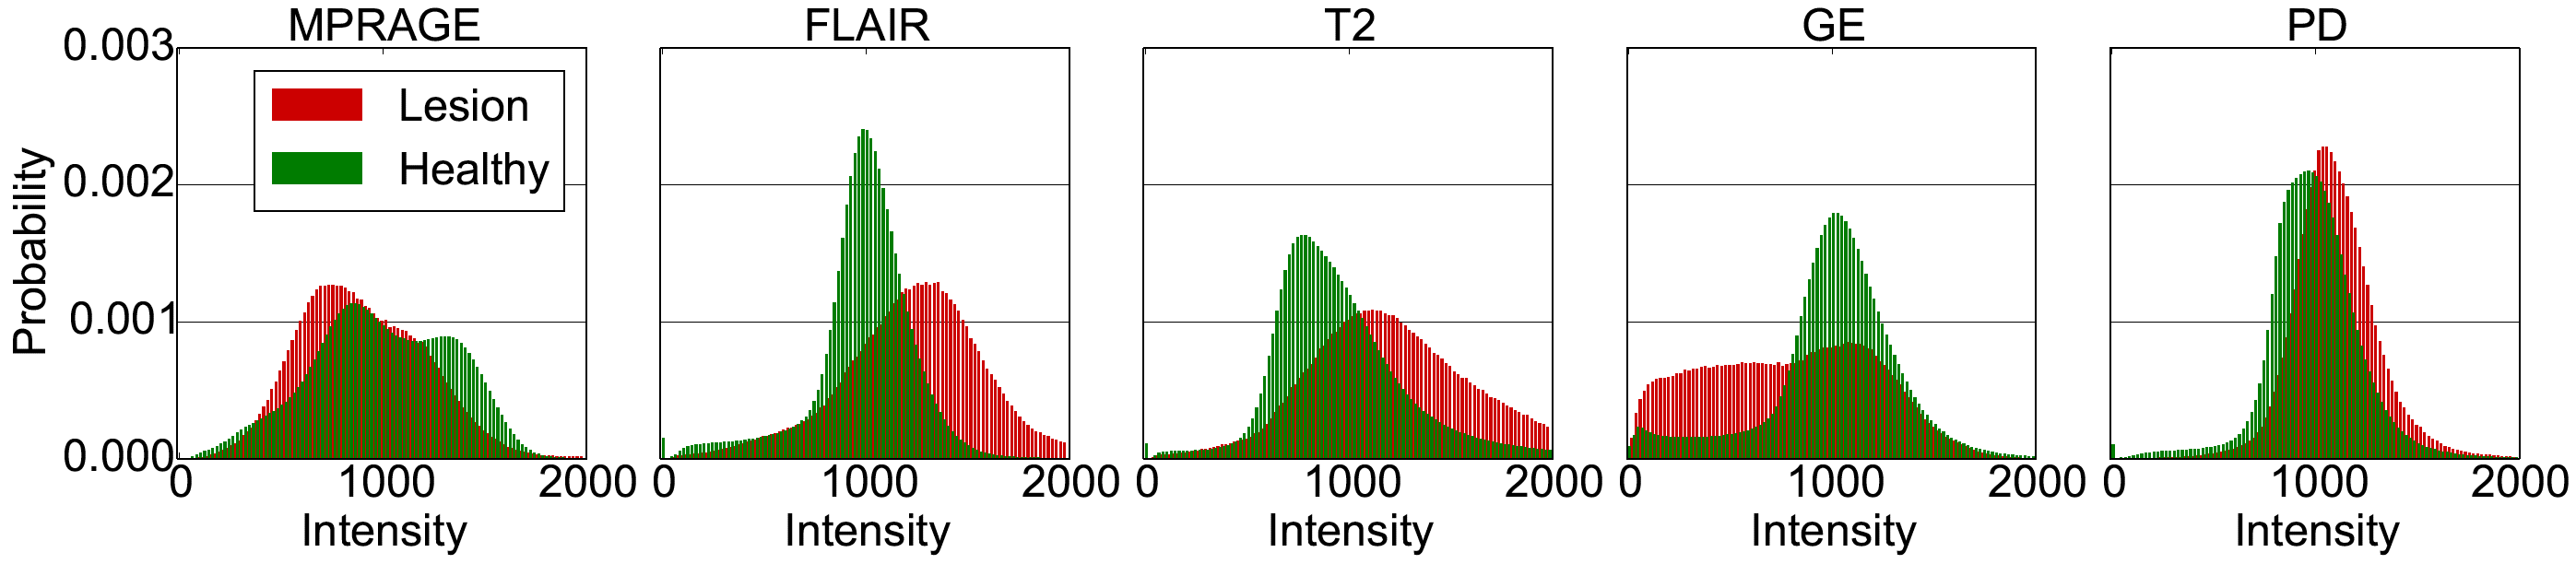
\includegraphics[clip=true, trim=0pt 0pt 0pt 0pt, width=1.0\textwidth]{figures/introduction/trio/intHistoTrio1_5mods.png}
	\caption{}
	\label{fig:histInt}
\end{subfigure}

\caption{Heterogeneous appearance of TBI lesions poses challenges in devising discriminative models. Lesion size varies significantly with both large, focal and small, diffused lesions (a,b). Alignment of manual lesion segmentations reveals the wide spatial distribution of lesions in (c,d) with some areas being more likely than others. (e) shows the average of the normalized intensity histograms of different MR channels over all the TBI cases in our database, for healthy (green) and injured (red) tissue. One can observe a large overlap between the distributions of healthy and non-healthy tissue.}
\label{fig:tbiChallenges}
\end{figure}